\chapter{2D case}

\section{Problem}
In this part, we will focus on a 2D point cloud and we will use for the energy
the area of the $r$-offset of a point cloud (the Minkowski sum with an euclidean
ball: $B(0, r)$ ).

\section{Area of a union of balls}
In order to compute this energy, we need to know how to estimate the area of the
intersection of a ball and a Voronoi cell.
This is the same work as the one done in \cite{cazals2011computing} except that
we restrict ourselves to 2D which is simpler than in 3D.

For doing that, we need to decompose the intersection into triangles and
spherical caps.

\begin{figure}[H]
   \centering
   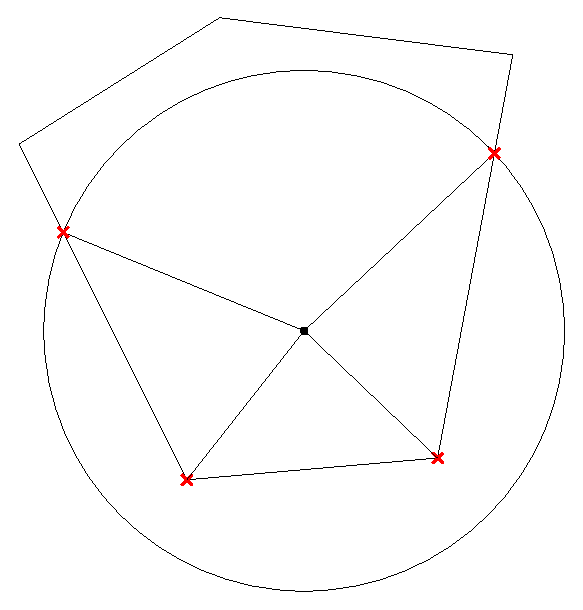
\includegraphics[width=0.3\hsize]{inter_voronoi_ball_2d}
   \caption{Different cases for the intersection between a Voronoi cell and a sphere}
   \label{fig:inter_voronoi_ball_2d}
\end{figure}

\section{Gradient descent}
We needed to choose "good" weights for the gradient descent. Indeed, in a normal
mean curvature flow, all the points move with the same distance. But here, this
may not be the case since the energy depends on the curvature of our restricted
region.

One way to avoid this problem is to weight the gradient by the perimeter of the
visible part of the restricted region. But by doing, we can divide by $0$ so we
need to choose the timestep according to these weights.

\section{Experiments}
We did some experiments to validate our results. The fist thing we did was to
apply our flow to a set of points randomly chosen on an ellipse.

Then, we added some noise on these points.

% Union of balls
% Intersection with Voronoi cells
% Volume
% Gradient descent: weights
% Experiments

% vim: set spelllang=en :
